% Options for packages loaded elsewhere
\PassOptionsToPackage{unicode}{hyperref}
\PassOptionsToPackage{hyphens}{url}
%
\documentclass[
]{article}
\usepackage{amsmath,amssymb}
\usepackage{iftex}
\ifPDFTeX
  \usepackage[T1]{fontenc}
  \usepackage[utf8]{inputenc}
  \usepackage{textcomp} % provide euro and other symbols
\else % if luatex or xetex
  \usepackage{unicode-math} % this also loads fontspec
  \defaultfontfeatures{Scale=MatchLowercase}
  \defaultfontfeatures[\rmfamily]{Ligatures=TeX,Scale=1}
\fi
\usepackage{lmodern}
\ifPDFTeX\else
  % xetex/luatex font selection
\fi
% Use upquote if available, for straight quotes in verbatim environments
\IfFileExists{upquote.sty}{\usepackage{upquote}}{}
\IfFileExists{microtype.sty}{% use microtype if available
  \usepackage[]{microtype}
  \UseMicrotypeSet[protrusion]{basicmath} % disable protrusion for tt fonts
}{}
\makeatletter
\@ifundefined{KOMAClassName}{% if non-KOMA class
  \IfFileExists{parskip.sty}{%
    \usepackage{parskip}
  }{% else
    \setlength{\parindent}{0pt}
    \setlength{\parskip}{6pt plus 2pt minus 1pt}}
}{% if KOMA class
  \KOMAoptions{parskip=half}}
\makeatother
\usepackage{xcolor}
\usepackage[margin=1in]{geometry}
\usepackage{longtable,booktabs,array}
\usepackage{calc} % for calculating minipage widths
% Correct order of tables after \paragraph or \subparagraph
\usepackage{etoolbox}
\makeatletter
\patchcmd\longtable{\par}{\if@noskipsec\mbox{}\fi\par}{}{}
\makeatother
% Allow footnotes in longtable head/foot
\IfFileExists{footnotehyper.sty}{\usepackage{footnotehyper}}{\usepackage{footnote}}
\makesavenoteenv{longtable}
\usepackage{graphicx}
\makeatletter
\def\maxwidth{\ifdim\Gin@nat@width>\linewidth\linewidth\else\Gin@nat@width\fi}
\def\maxheight{\ifdim\Gin@nat@height>\textheight\textheight\else\Gin@nat@height\fi}
\makeatother
% Scale images if necessary, so that they will not overflow the page
% margins by default, and it is still possible to overwrite the defaults
% using explicit options in \includegraphics[width, height, ...]{}
\setkeys{Gin}{width=\maxwidth,height=\maxheight,keepaspectratio}
% Set default figure placement to htbp
\makeatletter
\def\fps@figure{htbp}
\makeatother
\setlength{\emergencystretch}{3em} % prevent overfull lines
\providecommand{\tightlist}{%
  \setlength{\itemsep}{0pt}\setlength{\parskip}{0pt}}
\setcounter{secnumdepth}{5}
\usepackage{booktabs}
\usepackage{longtable}
\usepackage{lmodern}
\usepackage[T1]{fontenc}

\ifxetex
\usepackage{letltxmacro}
\setlength{\XeTeXLinkMargin}{1pt}
\LetLtxMacro\SavedIncludeGraphics\includegraphics
\def\includegraphics#1#{% #1 catches optional stuff (star/opt. arg.)
	\IncludeGraphicsAux{#1}%
}%
\newcommand*{\IncludeGraphicsAux}[2]{%
	\XeTeXLinkBox{%
		\SavedIncludeGraphics#1{#2}%
	}%
}%
\fi
\usepackage{flafter}
\usepackage{booktabs}
\usepackage{longtable}
\usepackage{array}
\usepackage{multirow}
\usepackage{wrapfig}
\usepackage{float}
\usepackage{colortbl}
\usepackage{pdflscape}
\usepackage{tabu}
\usepackage{threeparttable}
\usepackage{threeparttablex}
\usepackage[normalem]{ulem}
\usepackage{makecell}
\usepackage{xcolor}
\ifLuaTeX
  \usepackage{selnolig}  % disable illegal ligatures
\fi
\usepackage{bookmark}
\IfFileExists{xurl.sty}{\usepackage{xurl}}{} % add URL line breaks if available
\urlstyle{same}
\hypersetup{
  pdftitle={Eastern Zone 2023-2025 Size-limit Changes},
  pdfauthor={Jaime McAllister},
  hidelinks,
  pdfcreator={LaTeX via pandoc}}

\title{Eastern Zone 2023-2025 Size-limit Changes}
\author{Jaime McAllister}
\date{2024-07-20}

\begin{document}
\maketitle

{
\setcounter{tocdepth}{2}
\tableofcontents
}
\section{Background}\label{background}

Since 2019 a series of Size Limit changes have gradually been introduced to the fishery with the aim of providing three years of protection post reproductive maturity of abalone populations around Tasmania. That required an increase in the Legal Minimum Length (LML) for the Tasmanian Eastern Zone blacklip fishery from 138 mm to 145 mm. This increase in LML was scheduled to occur in three steps, with the first step (138 mm to 140mm)implemented in 2023. The second step (140 mm to 142 mm) in 2024, and third (142 mm to 145 mm) is scheduled for 2025.

Changing size limits is likely to affect abalone stocks in multiple ways. Increasing the LML will initially reduce exploitable biomass which is expected to have short-term effects on catch and catch rates, as well as long-term benefits such as increased stock and stock biomass. There is often an argument put forward that some populations are `stunted' and will never attain the sizes of an increased LML, consequently reducing available biomass and reduction in CPUE. As CPUE is a key component of the Harvest Control Rule (HCR) in the empirical Harvest Strategy (eHS), there is concern that this will result in a total allowable commercial catch (TACC) reduction in the year following the implementation of LML increase. This has been of particular concern in the Eastern Zone where it has been suggested the scheduled LML increase to 145 mm in Block 13 (Actaeon's Region) is too high and abalone will never attain these sizes.

Therefore the purpose of these analysis is to examine historical size structure trends in the Actaeon's region to assess the effect of LML increases on stock availability. The main objectives were to:

\begin{enumerate}
\def\labelenumi{\arabic{enumi}.}
\tightlist
\item
  Examine historical trends in size structure.
\item
  Examine recent length weight data to determine effect on abalone harvest numbers and biomass.
\end{enumerate}

\section{Size structure compositions}\label{size-structure-compositions}

\subsection{Historical size stucture 1984-2024}\label{historical-size-stucture-1984-2024}

Size composition data collected since 1984 has varied markedly between years. Catch compositions were comprised of a broader size distribution up until the early 2000s, however, since then have become increasingly dominated by animals between the LML and 155 mm (Figure \ref{fig:betweenyearsize}). In all years there is clearly evidence of large abalone \textgreater160 mm and in many cases animals in excess of 200 mm present in catches, and since 2010 the median size has regularly exceeded the the scheduled 145 mm LML increase.

\begin{figure}

{\centering 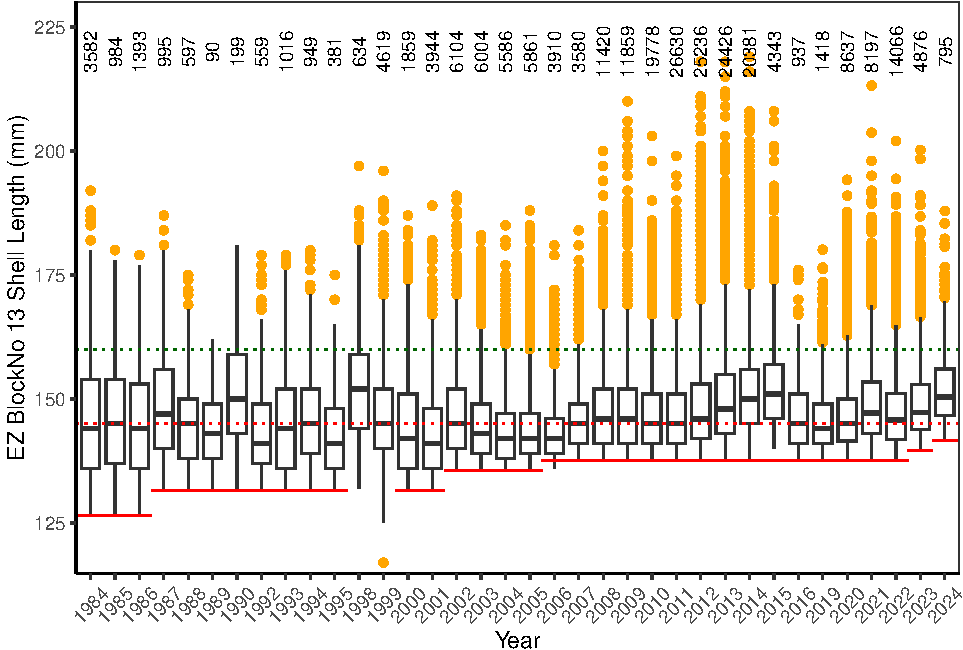
\includegraphics[width=0.8\textwidth,height=0.8\textwidth]{MM_Length-Weight_LML_final_test_files/figure-latex/betweenyearsize-1} 

}

\caption{Block 13 EZ: Boxplot of length frequency distributions between 1984 and 2024. Red line under each boxplot indicates LML for that year. Red dotted line represents LML = 145 mm; green dotted line denotes a shell length = 160 mm;  oranges dots are individual abalone measurments (outliers). Number of abalone measured given above each boxplot.}\label{fig:betweenyearsize}
\end{figure}

\subsection{Percentage contribution of scheduled LML changes to catch}\label{percentage-contribution-of-scheduled-lml-changes-to-catch}

A breakdown of historical catch compositions into the scheduled LML changes in the Eastern Zone demonstrates that catches have been dominated by at least 50\% of abalone being \textgreater145 mm throughout time series (Figure \ref{fig:betweenyearsize}). Cycles in recruitment are also apparent with a significant period of re-build and recruitment occurring during the mid 2000s demonstrated by a higher proportion of smaller individuals dominating catches (Figure \ref{fig:sizecontribution}). A similar pattern of recruitment has also occurred in recent years with an apparent pulse of smaller individuals entering the fishery around 2019 which have since progressed to dominate catches as larger individuals in latter years (Figure \ref{fig:sizecontribution}).

\begin{figure}

{\centering 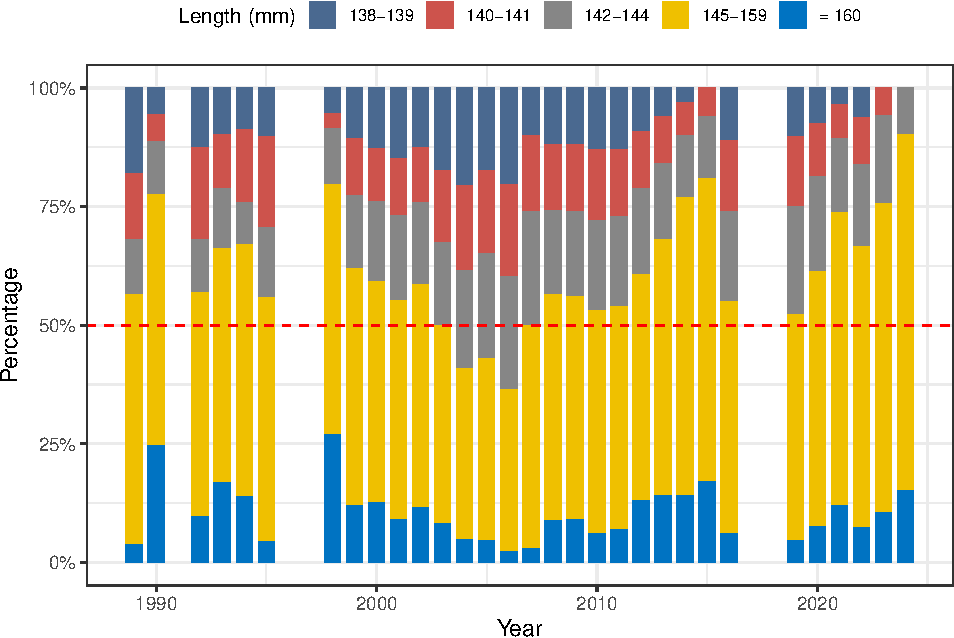
\includegraphics[width=0.8\textwidth,height=0.8\textwidth]{MM_Length-Weight_LML_final_test_files/figure-latex/sizecontribution-1} 

}

\caption{Block 13 EZ: Percentage contribution of size classes to commercial abalone catches collected between 2019-2024.}\label{fig:sizecontribution}
\end{figure}

\section{Size structure 2019-2024}\label{size-structure-2019-2024}

Further examination of more recent size composition data between 2019 and 2024 shows the majority of catches have been dominated by animals between the LML and 155 mm (Figure \ref{fig:yearlengthfrequency}). Whilst there are clearly animals still reaching \textgreater160 mm the fishery has largely become recruitment driven and catches dominated by animals \textless160 mm. However, these recent catches (2019-2024) appear to have been dominated by a single cohort from an initial recruitment pulse around 2019, evidenced by an increasing median size and absence of animals nearer to the LML. These trends suggest there has likely been a recruitment gap year sometime in fishery since around 2019 and has resulted in a higher dependence on animals that have attained larger sizes. Consequently, this is likely to contribute towards lower catch rates given there have generally been fewer animals reaching these larger sizes in more recent years.

\begin{figure}

{\centering 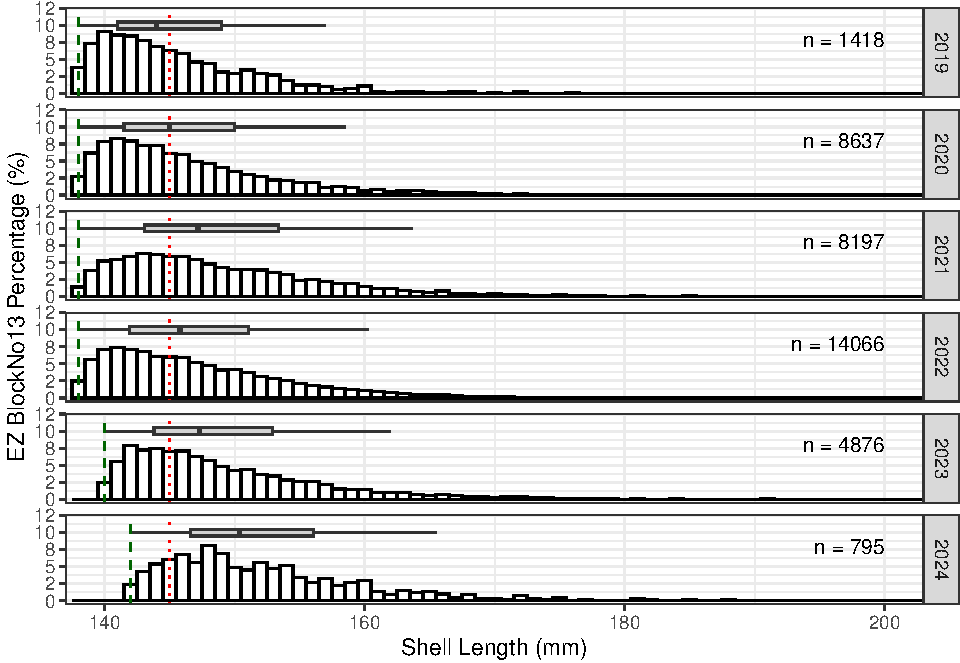
\includegraphics[width=0.8\textwidth,height=0.8\textwidth]{MM_Length-Weight_LML_final_test_files/figure-latex/yearlengthfrequency-1} 

}

\caption{Block 13 EZ: Length frequency distributions between 2019 and 2024. Green dashed line indicates LML for that year; red dotted line indicates LML = 145 mm. n = number of abalone measured.}\label{fig:yearlengthfrequency}
\end{figure}

\subsection{Within year size composition}\label{within-year-size-composition}

Abalone populations are spatially dynamic and can vary in size structure across small spatial distances (i.e.~10s to 100s metres). Productivity is therefore highly variable across reefs which in turn can determine the spatial distribution of fishing effort and rate of harvest. More productive, faster growing areas tend to be fished more regularly whereas less effort may be directed towards slower growing and less productive areas. Therefore it is not surprising that within a fishing year (2023) there is high variability in size structure between catches from the Actaeons (Figure \ref{fig:fishyearsize}). Whilst the precise spatial locations of those catches measured has not been examined it is interesting to note that in 93\% of catches, the median size of animals was \textgreater145 mm and in every catch there was at least one animal \textgreater158 mm. Whilst further examination of spatial fishing data is required to determine the distribution of catch measurement locations, there is a high probability that at least some of these catches were measured from areas considered to be of low productivity, highlighting that growth is not limited by their environment, rather likely constrained by excessive fishing pressure and limiting the time animals have to reach larger sizes before they are harvested.

\begin{figure}

{\centering 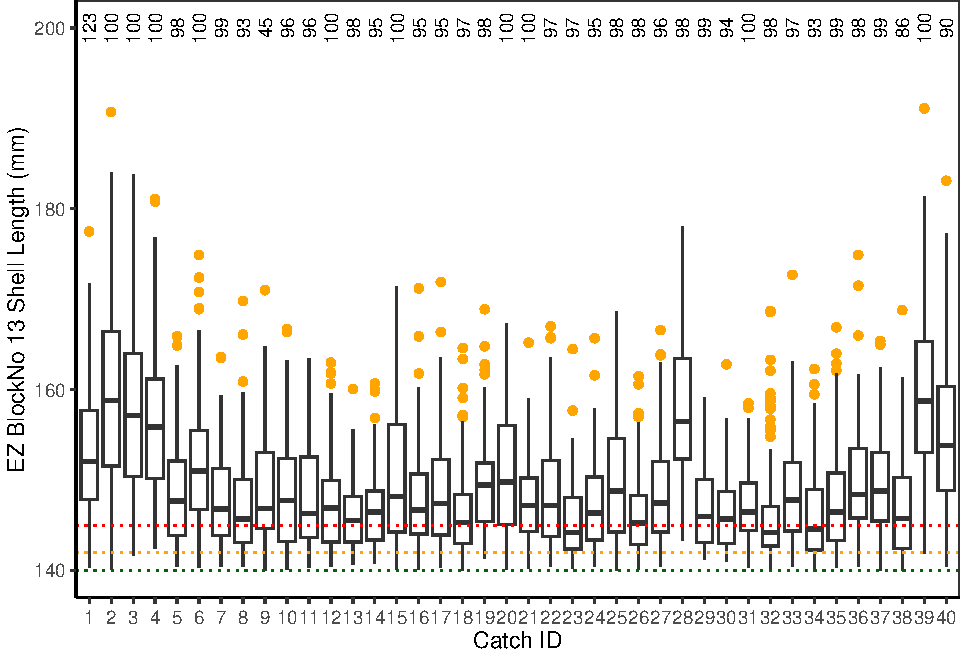
\includegraphics[width=0.8\textwidth,height=0.8\textwidth]{MM_Length-Weight_LML_final_test_files/figure-latex/fishyearsize-1} 

}

\caption{Block 13 EZ: Range of size compositions between individual commercial abalone catches collected in 2023.}\label{fig:fishyearsize}
\end{figure}

\section{Length-weight relationship 2019-2024}\label{length-weight-relationship-2019-2024}

\subsection{Background}\label{background-1}

Length and weight data have been collected concurrently since 2019 using Scielex NextGen measuring boards with integrated platform scales at various abalone processing factories around Tasmania. This is providing an improved understanding of stock performance and abalone condition across many parts of the fishery whilst also facilitating processors with grading and handling information on processed catches. Importantly these data have enabled a refinement of length-weight relationships for stock assessments which are used here for translating catch composition in terms of catch numbers to weight estimates in assessing the effects of size limit changes to landed biomass.

\subsection{Length-weight data prepartion}\label{length-weight-data-prepartion}

\subsubsection{Length-weight data filtering}\label{length-weight-data-filtering}

An initial plot of all length and weight data collected since 2019 to look for any obvious data outliers (Figure \ref{fig:lwdatacheck}). There are clearly several erroneous length and weight data collected in the initial plot and can be attributed to:

\begin{enumerate}
\def\labelenumi{\arabic{enumi}.}
\tightlist
\item
  Abalone weights \textless200 g or \textgreater1500 g are highly unlikely.
\item
  Calibration and practice measurements taken at the default return position of
  the measuring gates (i.e.~100 mm).
\item
  Measurement errors caused by operator error where animals are below the LML for a particular
  Zone especially where the measurement is \textgreater5 mm below the LML (e.g.~animals being measured
  shell side down or passed through the gates at an angle).
\item
  Failure to tare scales and abalone weights unlikely to correspond to appropriate
  length depending on the Zone (e.g.~EZ - shell length \textgreater{} 175 mm and whole weight \textless600 g; shell length \textgreater{} 180 mm and whole weight \textless1000 g).
\end{enumerate}

\begin{figure}

{\centering 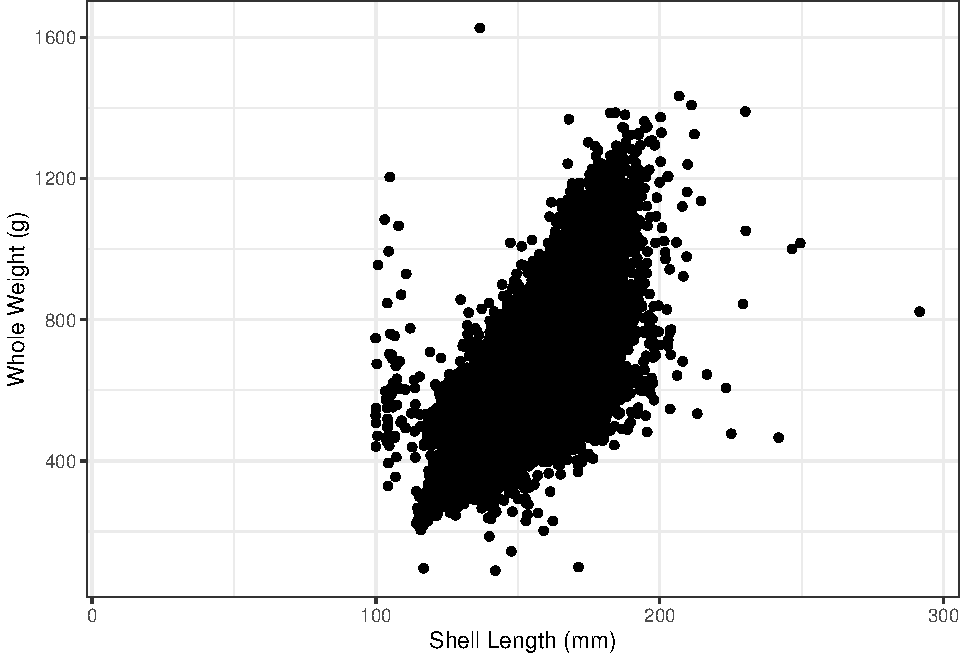
\includegraphics[width=0.8\textwidth,height=0.8\textwidth]{MM_Length-Weight_LML_final_test_files/figure-latex/lwdatacheck-1} 

}

\caption{Length-weight relationship of all commercial abalone catch sampling data collected between 2019-2024.}\label{fig:lwdatacheck}
\end{figure}

\subsubsection{Summary of available length-weight data for Zone and Block}\label{summary-of-available-length-weight-data-for-zone-and-block}

Summary of catches measured in chosen Zone and Block where the catch can be assigned to a single Block (i.e.~only a single Block listed on Docket) (Table \ref{tab:catchsamplesbyblock}).

\begin{table}

\caption{\label{tab:catchsamplesbyblock}Block 13 EZ: Summary of catches measured from commercial abalone catch sampling data collected between 2019-2024.}
\centering
\begin{tabular}[t]{ccccc}
\toprule
\makecell[c]{Fishing\\Year} & Catches & n & \makecell[c]{Mean\\Length\\(mm)} & \makecell[c]{Mean\\Weight\\(g)}\\
\midrule
2019 & 10 & 912 & 146 & 510\\
2020 & 45 & 3966 & 148 & 565\\
2021 & 83 & 8040 & 149 & 550\\
2022 & 96 & 9244 & 147 & 551\\
2023 & 40 & 3765 & 150 & 582\\
2024 & 10 & 767 & 152 & 595\\
\bottomrule
\end{tabular}
\end{table}

\subsubsection{Selected Zone and Block data filtering}\label{selected-zone-and-block-data-filtering}

Re-examining the length and weight data collected since 2019 to look for any remaining data outliers that may be specific to this region (Figure \ref{fig:rechecklwdata}). For the Actaeon's there are specific erroneous data which are apparent based on known size and likely weights, shell length \textgreater175 mm and whole weight \textless600 g, or shell length \textgreater180 mm and whole weight \textless1000 g are likely to be measuring board operator errors and the failure to tare the platform scales. Removal of these data can be seen in cleaned length-weight relationship plot (Figure \ref{fig:cleanlwdata}).

\begin{figure}

{\centering 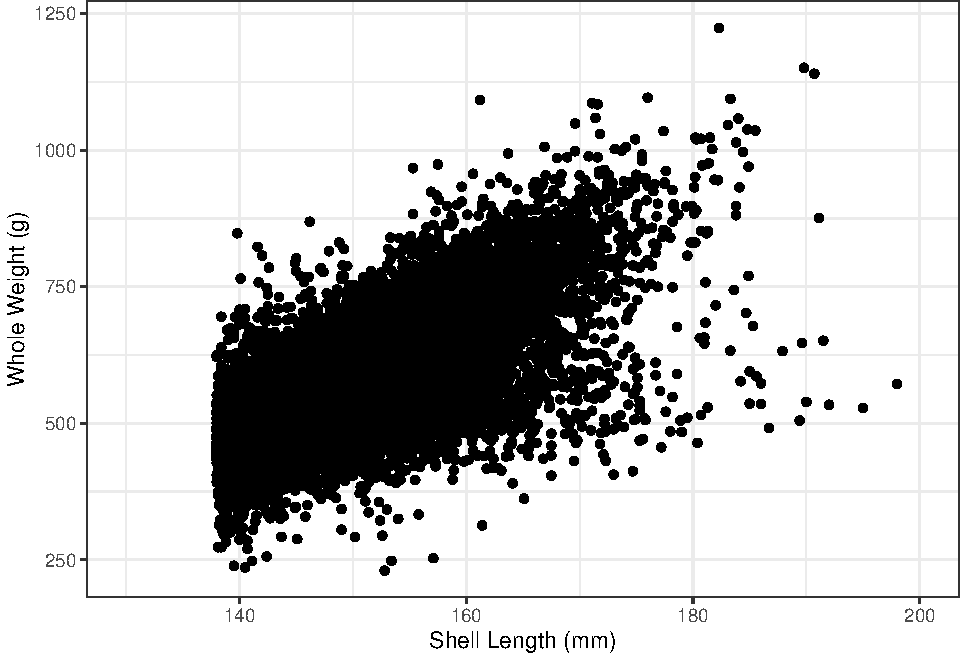
\includegraphics[width=0.8\textwidth,height=0.8\textwidth]{MM_Length-Weight_LML_final_test_files/figure-latex/rechecklwdata-1} 

}

\caption{Block 13 EZ: Length-weight relationship of commercial abalone catch sampling data collected between 2019-2024.}\label{fig:rechecklwdata}
\end{figure}

\begin{figure}

{\centering 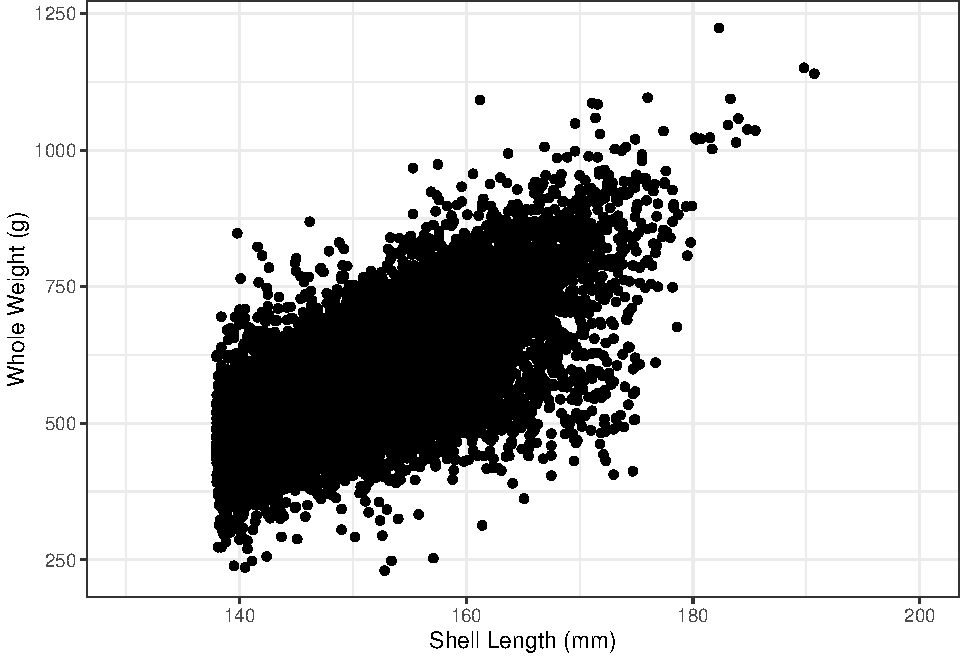
\includegraphics[width=0.8\textwidth,height=0.8\textwidth]{MM_Length-Weight_LML_final_test_files/figure-latex/cleanlwdata-1} 

}

\caption{Block 13 EZ: Length-weight relationship of cleaned commercial abalone catch sampling data collected between 2019-2024.}\label{fig:cleanlwdata}
\end{figure}

\subsection{Calculation of length-weight relationships}\label{calculation-of-length-weight-relationships}

The LML increases will create an initial reduction in available biomass and affect the number of abalone handled until individuals grow through to the new LML. Whilst it is evident from length composition data 61\% of abalone measured each year during the period 2019-2024 were on average \textgreater145 mm, in order to evaluate how the LML increases may affect harvested biomass and ultimately catch rates (kg/hr), a length-weight relationship was required.

\subsection{Calculate length-weight relationship for selected Zone and Block}\label{calculate-length-weight-relationship-for-selected-zone-and-block}

The length-weight relationship was calculated by fitting the data to a two-parameter power function of the form

\(W_{i} = aL_{i}^{b}\) (1)

where \emph{a} and \emph{b} are constants. The length-weight model (1)can be transformed to a linear model by taking the natural logarithms of both sides and simplifying,

\(\log(W_{i}) = \log(a) + \log(L_{i})\) (2)

Thus, with \emph{y=log(W)}, \emph{x=log(L)}, slope=\emph{b}, and intercept=\emph{log(a)}, (2) is in the form of a linear model. The transformed model is then fit with \emph{lm()} by submitting a formula of the form \emph{y\textasciitilde x} as the first argument followed by a \emph{data=} argument set equal to the data frame where the log-tranformed variables can be found.

\begin{table}

\caption{\label{tab:lengthweightrelationship}Block 13 EZ: Estimated length-weight model parameters from commercial abalone catch sampling data collected between 2019-2024.}
\centering
\begin{tabular}[t]{ccccc}
\toprule
Zone & BlockNo & a & b & n\\
\midrule
E & 13 & 0.0053805 & 2.307653 & 26625\\
\bottomrule
\end{tabular}
\end{table}

\subsection{Calculate percent contribution of abalone by weight and numbers}\label{calculate-percent-contribution-of-abalone-by-weight-and-numbers}

The calculated length-weight model parameters for the Zone and Block were used to estimate the individual abalone weight for each 1 mm size class above the previous LML (i.e.~138 mm). The estimated size class weight was then multiplied by the total number of individuals measured to determine the total weight of that size class. The estimated total weight and numbers measured were then used to determine the percentage by weight and numbers of that size class to the overall size composition data.

\begin{longtable}[t]{cccccc}
\caption{\label{tab:weightnumbercontribution}Block 13 EZ: Estimated percentage contribution of each 1 mm size class by weight and numbers using length-weight model parameters from commercial abalone catch sampling data collected between 2019-2024\textit{ (a = 0.00538; b = 2.308).}}\\
\toprule
\makecell[c]{Shell\\Length\\(mm)} & \makecell[c]{Estimated\\Weight\\(g)} & n & \makecell[c]{Catch\\Weight\\(kg)} & \makecell[c]{Percent\\n} & \makecell[c]{Percent\\Weight}\\
\midrule
138 & 466.6 & 790 & 369 & 2.959 & 2.513\\
139 & 474.4 & 1236 & 586 & 4.630 & 3.990\\
140 & 482.3 & 1579 & 762 & 5.915 & 5.189\\
141 & 490.3 & 1703 & 835 & 6.380 & 5.686\\
142 & 498.4 & 1766 & 880 & 6.616 & 5.992\\
143 & 506.5 & 1751 & 887 & 6.560 & 6.040\\
144 & 514.7 & 1684 & 867 & 6.309 & 5.904\\
145 & 523.0 & 1637 & 856 & 6.132 & 5.829\\
146 & 531.4 & 1564 & 831 & 5.859 & 5.658\\
147 & 539.8 & 1373 & 741 & 5.143 & 5.046\\
148 & 548.3 & 1317 & 722 & 4.934 & 4.916\\
149 & 556.9 & 1120 & 624 & 4.196 & 4.249\\
150 & 565.6 & 1072 & 606 & 4.016 & 4.126\\
151 & 574.3 & 983 & 565 & 3.682 & 3.847\\
152 & 583.1 & 897 & 523 & 3.360 & 3.561\\
153 & 592.0 & 856 & 507 & 3.207 & 3.452\\
154 & 601.0 & 692 & 416 & 2.592 & 2.833\\
155 & 610.0 & 624 & 381 & 2.338 & 2.594\\
156 & 619.1 & 583 & 361 & 2.184 & 2.458\\
157 & 628.3 & 471 & 296 & 1.764 & 2.016\\
158 & 637.6 & 415 & 265 & 1.555 & 1.804\\
159 & 647.0 & 419 & 271 & 1.570 & 1.845\\
160 & 656.4 & 311 & 204 & 1.165 & 1.389\\
161 & 665.9 & 257 & 171 & 0.963 & 1.164\\
162 & 675.5 & 228 & 154 & 0.854 & 1.049\\
163 & 685.1 & 226 & 155 & 0.847 & 1.055\\
164 & 694.9 & 170 & 118 & 0.637 & 0.803\\
165 & 704.7 & 156 & 110 & 0.584 & 0.749\\
166 & 714.6 & 129 & 92 & 0.483 & 0.626\\
167 & 724.6 & 110 & 80 & 0.412 & 0.545\\
168 & 734.6 & 103 & 76 & 0.386 & 0.517\\
169 & 744.7 & 72 & 54 & 0.270 & 0.368\\
170 & 755.0 & 74 & 56 & 0.277 & 0.381\\
171 & 765.2 & 64 & 49 & 0.240 & 0.334\\
172 & 775.6 & 50 & 39 & 0.187 & 0.266\\
173 & 786.1 & 39 & 31 & 0.146 & 0.211\\
174 & 796.6 & 32 & 25 & 0.120 & 0.170\\
175 & 807.2 & 30 & 24 & 0.112 & 0.163\\
176 & 817.9 & 18 & 15 & 0.067 & 0.102\\
177 & 828.6 & 11 & 9 & 0.041 & 0.061\\
178 & 839.5 & 12 & 10 & 0.045 & 0.068\\
179 & 850.4 & 6 & 5 & 0.022 & 0.034\\
180 & 861.4 & 13 & 11 & 0.049 & 0.075\\
181 & 872.5 & 12 & 10 & 0.045 & 0.068\\
182 & 883.7 & 3 & 3 & 0.011 & 0.020\\
183 & 894.9 & 7 & 6 & 0.026 & 0.041\\
184 & 906.2 & 8 & 7 & 0.030 & 0.048\\
185 & 917.6 & 5 & 5 & 0.019 & 0.034\\
186 & 929.1 & 3 & 3 & 0.011 & 0.020\\
187 & 940.7 & 1 & 1 & 0.004 & 0.007\\
189 & 964.1 & 3 & 3 & 0.011 & 0.020\\
190 & 975.9 & 2 & 2 & 0.007 & 0.014\\
191 & 987.8 & 2 & 2 & 0.007 & 0.014\\
192 & 999.7 & 1 & 1 & 0.004 & 0.007\\
195 & 1036.2 & 1 & 1 & 0.004 & 0.007\\
198 & 1073.3 & 1 & 1 & 0.004 & 0.007\\
203 & 1136.9 & 1 & 1 & 0.004 & 0.007\\
213 & 1270.3 & 1 & 1 & 0.004 & 0.007\\
\bottomrule
\end{longtable}

\section{Results}\label{results}

\subsection{Percentage contribution of scheduled LML increases to catch}\label{percentage-contribution-of-scheduled-lml-increases-to-catch}

Overall there would be a 35\% reduction to exploitable biomass and 40\% reduction in catch numbers resulting from the LML increase from 138 mm to 145 mm (Table \ref{tab:lmlsumtab}). However, this assumes

Approx 60\% of catch since 2019 has been larger than scheduled maximum LML increase to 145 mm in 2025.

\begin{table}

\caption{\label{tab:lmlsumtab}Block 13 EZ: Estimated percentage contribution of abalone by weight and numbers to size classes representing the scheduled LML increases for using length-weight model parameters from commercial abalone catch sampling data collected between 2019-2024\textit{ (a = 0.00538; b = 2.308).}}
\centering
\begin{tabular}[t]{ccc}
\toprule
\makecell[c]{Size Class\\(mm)} & \makecell[c]{Percent\\Weight} & \makecell[c]{Percent\\n}\\
\midrule
138-139 mm & 6.5 & 7.6\\
140-141 mm & 10.9 & 12.3\\
142-144 mm & 17.9 & 19.5\\
$\geq$ 145 mm & 64.7 & 60.6\\
\bottomrule
\end{tabular}
\end{table}

\end{document}
